\documentclass{standalone}
%
\usepackage{tikz}
\usetikzlibrary{backgrounds,shapes.callouts}
\tikzstyle directed=[postaction={decorate,decoration={markings, mark=at position .5 with {\arrow{>}}}}]
\usepackage{tkz-euclide}
\usepackage{xcolor}
\usepackage{ifthen}
%
\definecolor{space}{HTML}{1F2C4E}
\definecolor{earth}{HTML}{0089FA}
\definecolor{dida}{HTML}{FFDE00}
\definecolor{title}{HTML}{FBA706}
\definecolor{moon}{HTML}{AFAFAF}
\definecolor{craterm}{HTML}{616060}
\definecolor{linem}{HTML}{DBDBDB}
\definecolor{core2}{HTML}{FF9616}
\definecolor{mars}{HTML}{DC7B4E}
%
\usepackage{fontspec}
\setmainfont{Open Dyslexic}
%
\title{Storia della misura della distanza Terra-Luna}
\begin{document}
	\tikzset{
		partial ellipse/.style args = {#1:#2:#3}{insert path={+ (#1:#3) arc (#1:#2:#3)}},
		notice/.style  = { draw, ellipse callout, callout relative pointer={#1} },
	}
	\begin{tikzpicture}[background rectangle/.style={fill=white},show background rectangle,>={[inset=0,angle'=27]Stealth}]
		\draw [use as bounding box, color=white] (-0.1,2.7) -| (30.2,2.7) |- (30.2,-118) -| (-0.1,-118);
		%title
		\begin{scope}%[shift={(0,15)}]
			\draw [black,ultra thick,fill=title] (0,-2.5) rectangle (30,2.5);
			\node (example-textwidth-2) [right, align=center, text width=35cm, color=black, font=\fontsize{60pt}{61pt}\selectfont] at (-3,0) {Storia della misura della distanza Terra-Luna};
		\end{scope}
		%
		\begin{scope}[shift={(0,-7.5)}]
			\node at (23,0) {
\includegraphics[width=5cm]{carl_sagan}};
			\node (example-textwidth-2) [notice={(3,0.5)}, ultra thick, right, align=center, text width=12cm, color=black, fill=white, font=\fontsize{23pt}{24pt}\selectfont] at (1,-1) {I metodi più antichi sono quello dell'eclissi lunare, come fatto da \textbf{Aristarco di Samo} nel IV secolo a.C. e successivamente da \textbf{Ipparco da Samo}. Quest'ultimo ottenne un risultato compreso tra i 376000 e i 427000 km.};
		\end{scope}
		%
		\begin{scope}[shift={(0,-17.5)}]
			\node at (7,0) {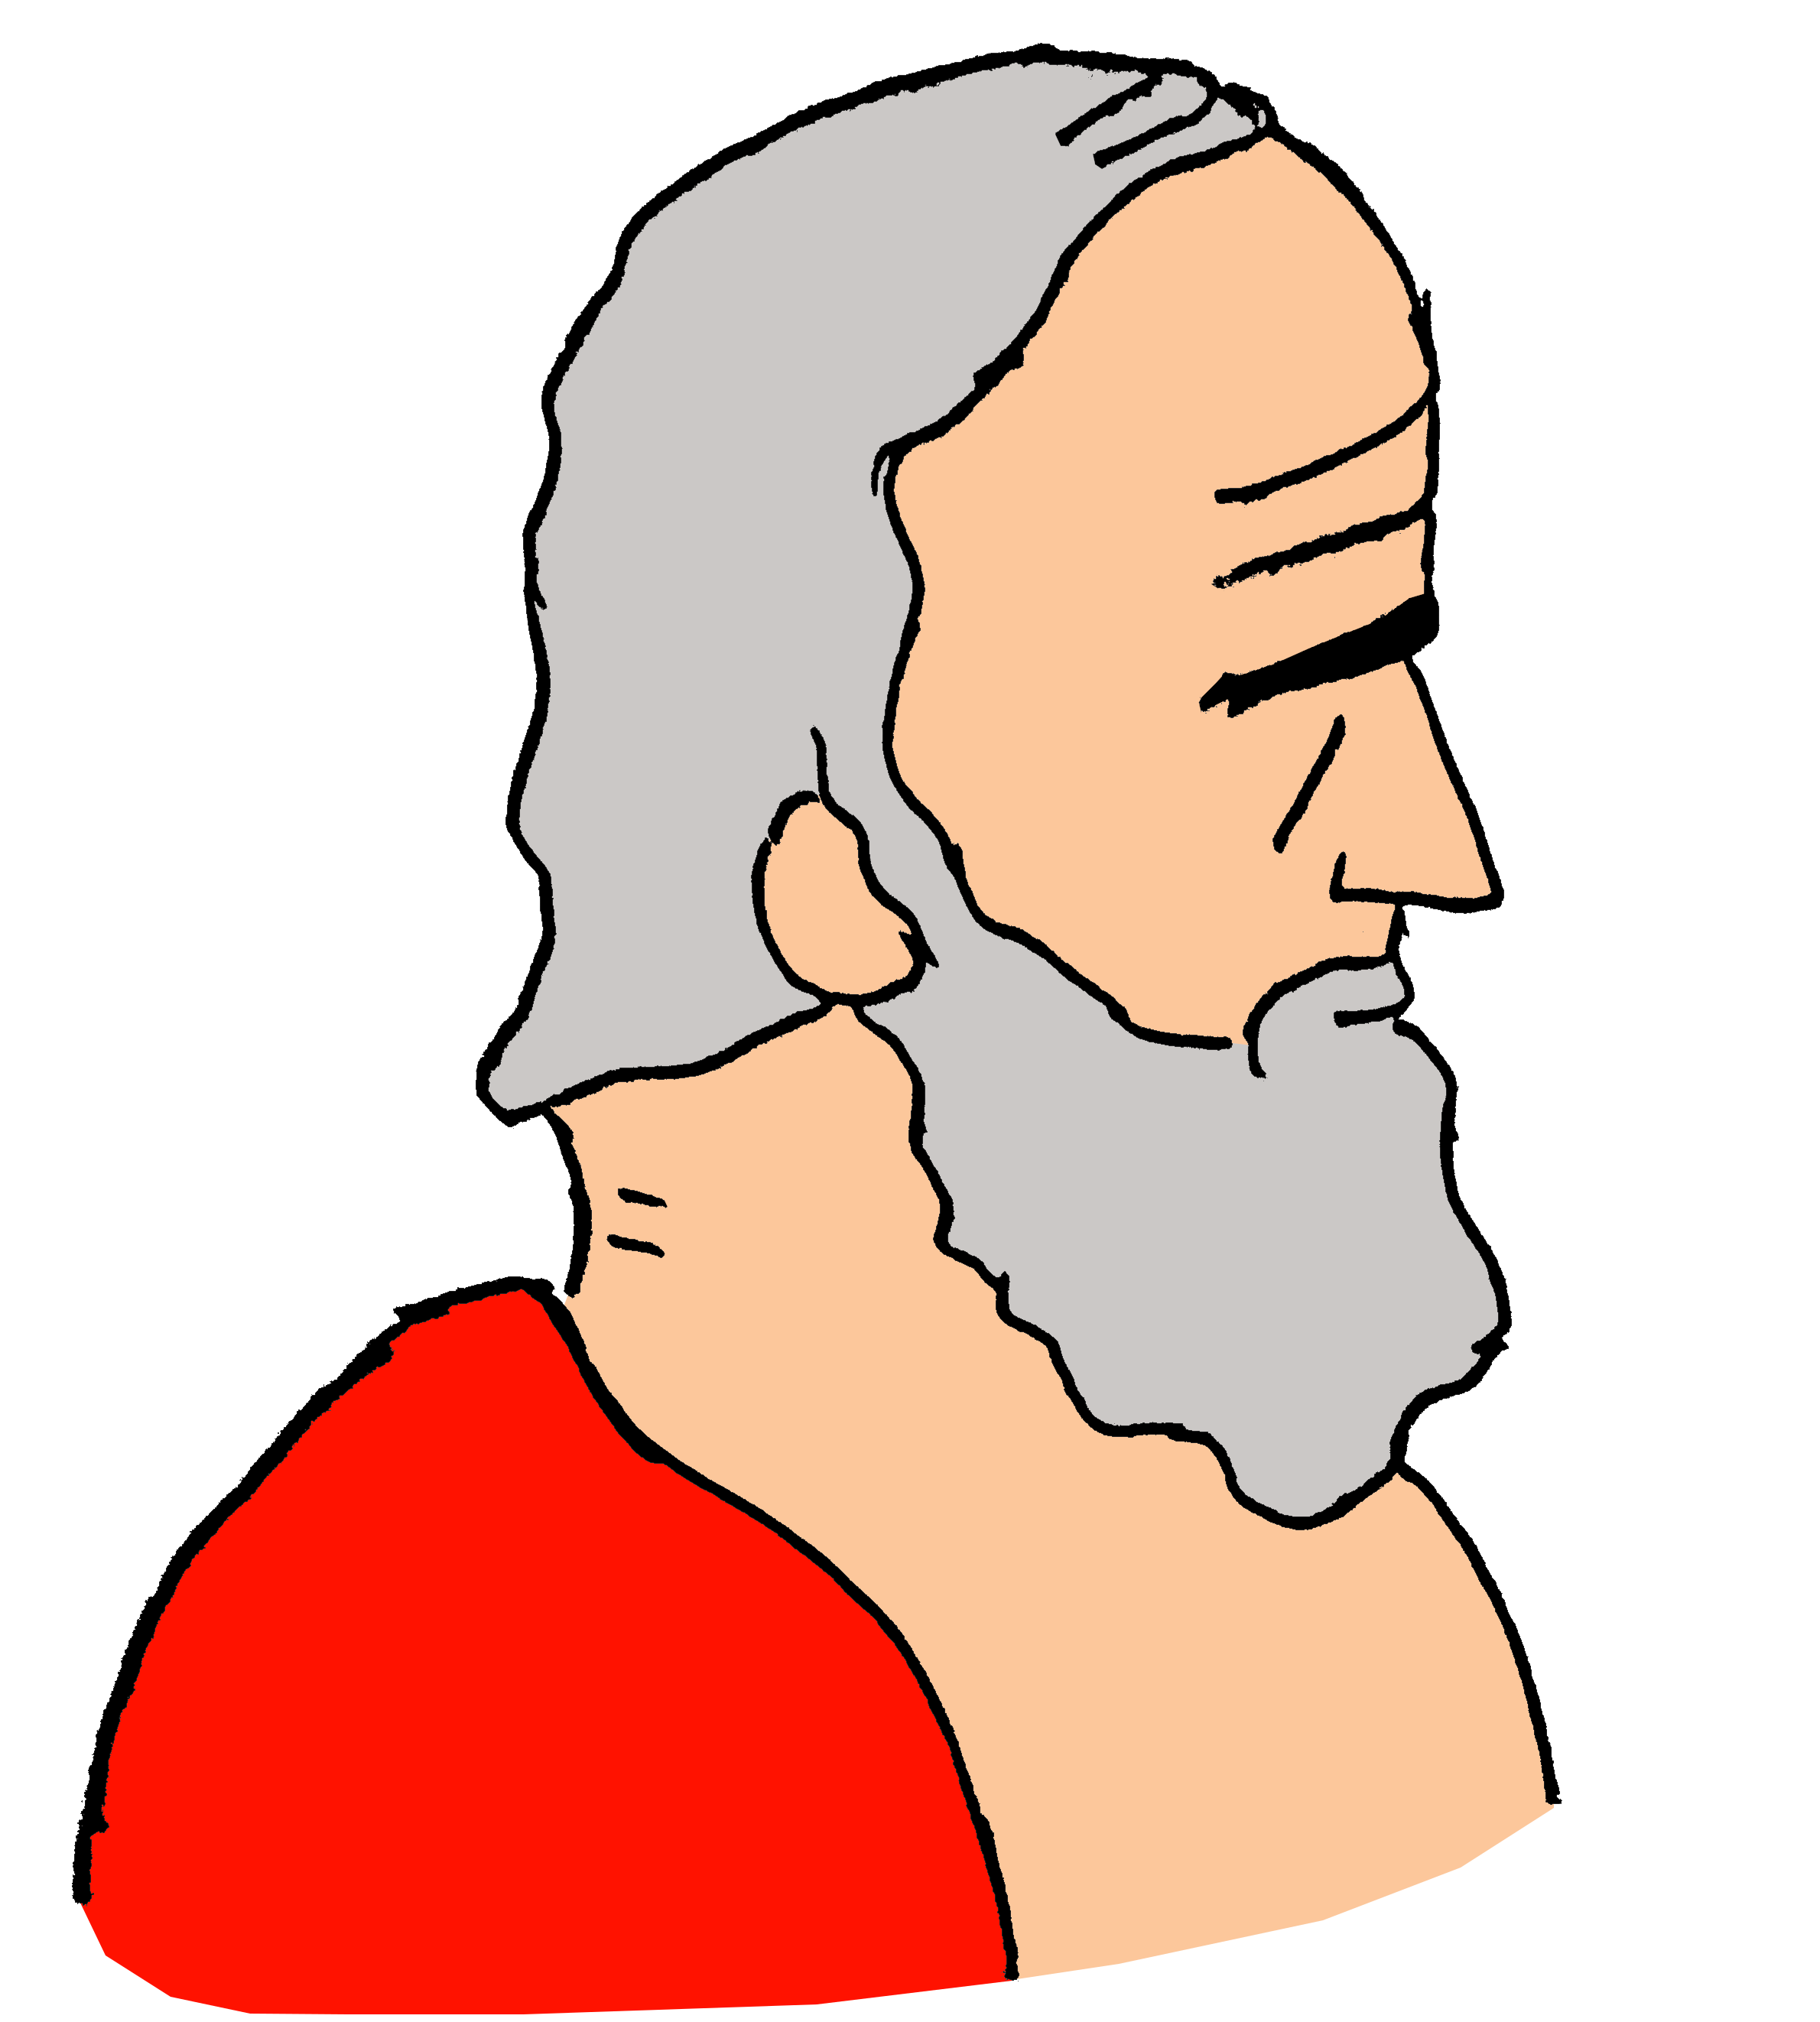
\includegraphics[width=8cm]{ipparco}};
			\node (example-textwidth-2) [notice={(-3,0.5)}, ultra thick, right, align=center, text width=12cm, color=black, fill=white, font=\fontsize{23pt}{24pt}\selectfont] at (12,-1) {Purtroppo commisi alcuni errori, tanto che la misura che doveva essere una stima inferiore di tale distanza risultò maggiore rispetto a quella che doveva essere la stima superiore...};
		\end{scope}
		%
		\begin{scope}[shift={(0,-26)}]
			\node at (23,0) {
\includegraphics[width=5cm]{carl_sagan}};
			\node (example-textwidth-2) [notice={(3,0.5)}, ultra thick, right, align=center, text width=12cm, color=black, fill=white, font=\fontsize{23pt}{24pt}\selectfont] at (1,-1) {\textbf{Tolomeo}, a partire dai risultati di Ipparco, determinò una distanza di 409000 km.};
		\end{scope}
		%
		\begin{scope}[shift={(0,-34)}]
			\node at (7,0) {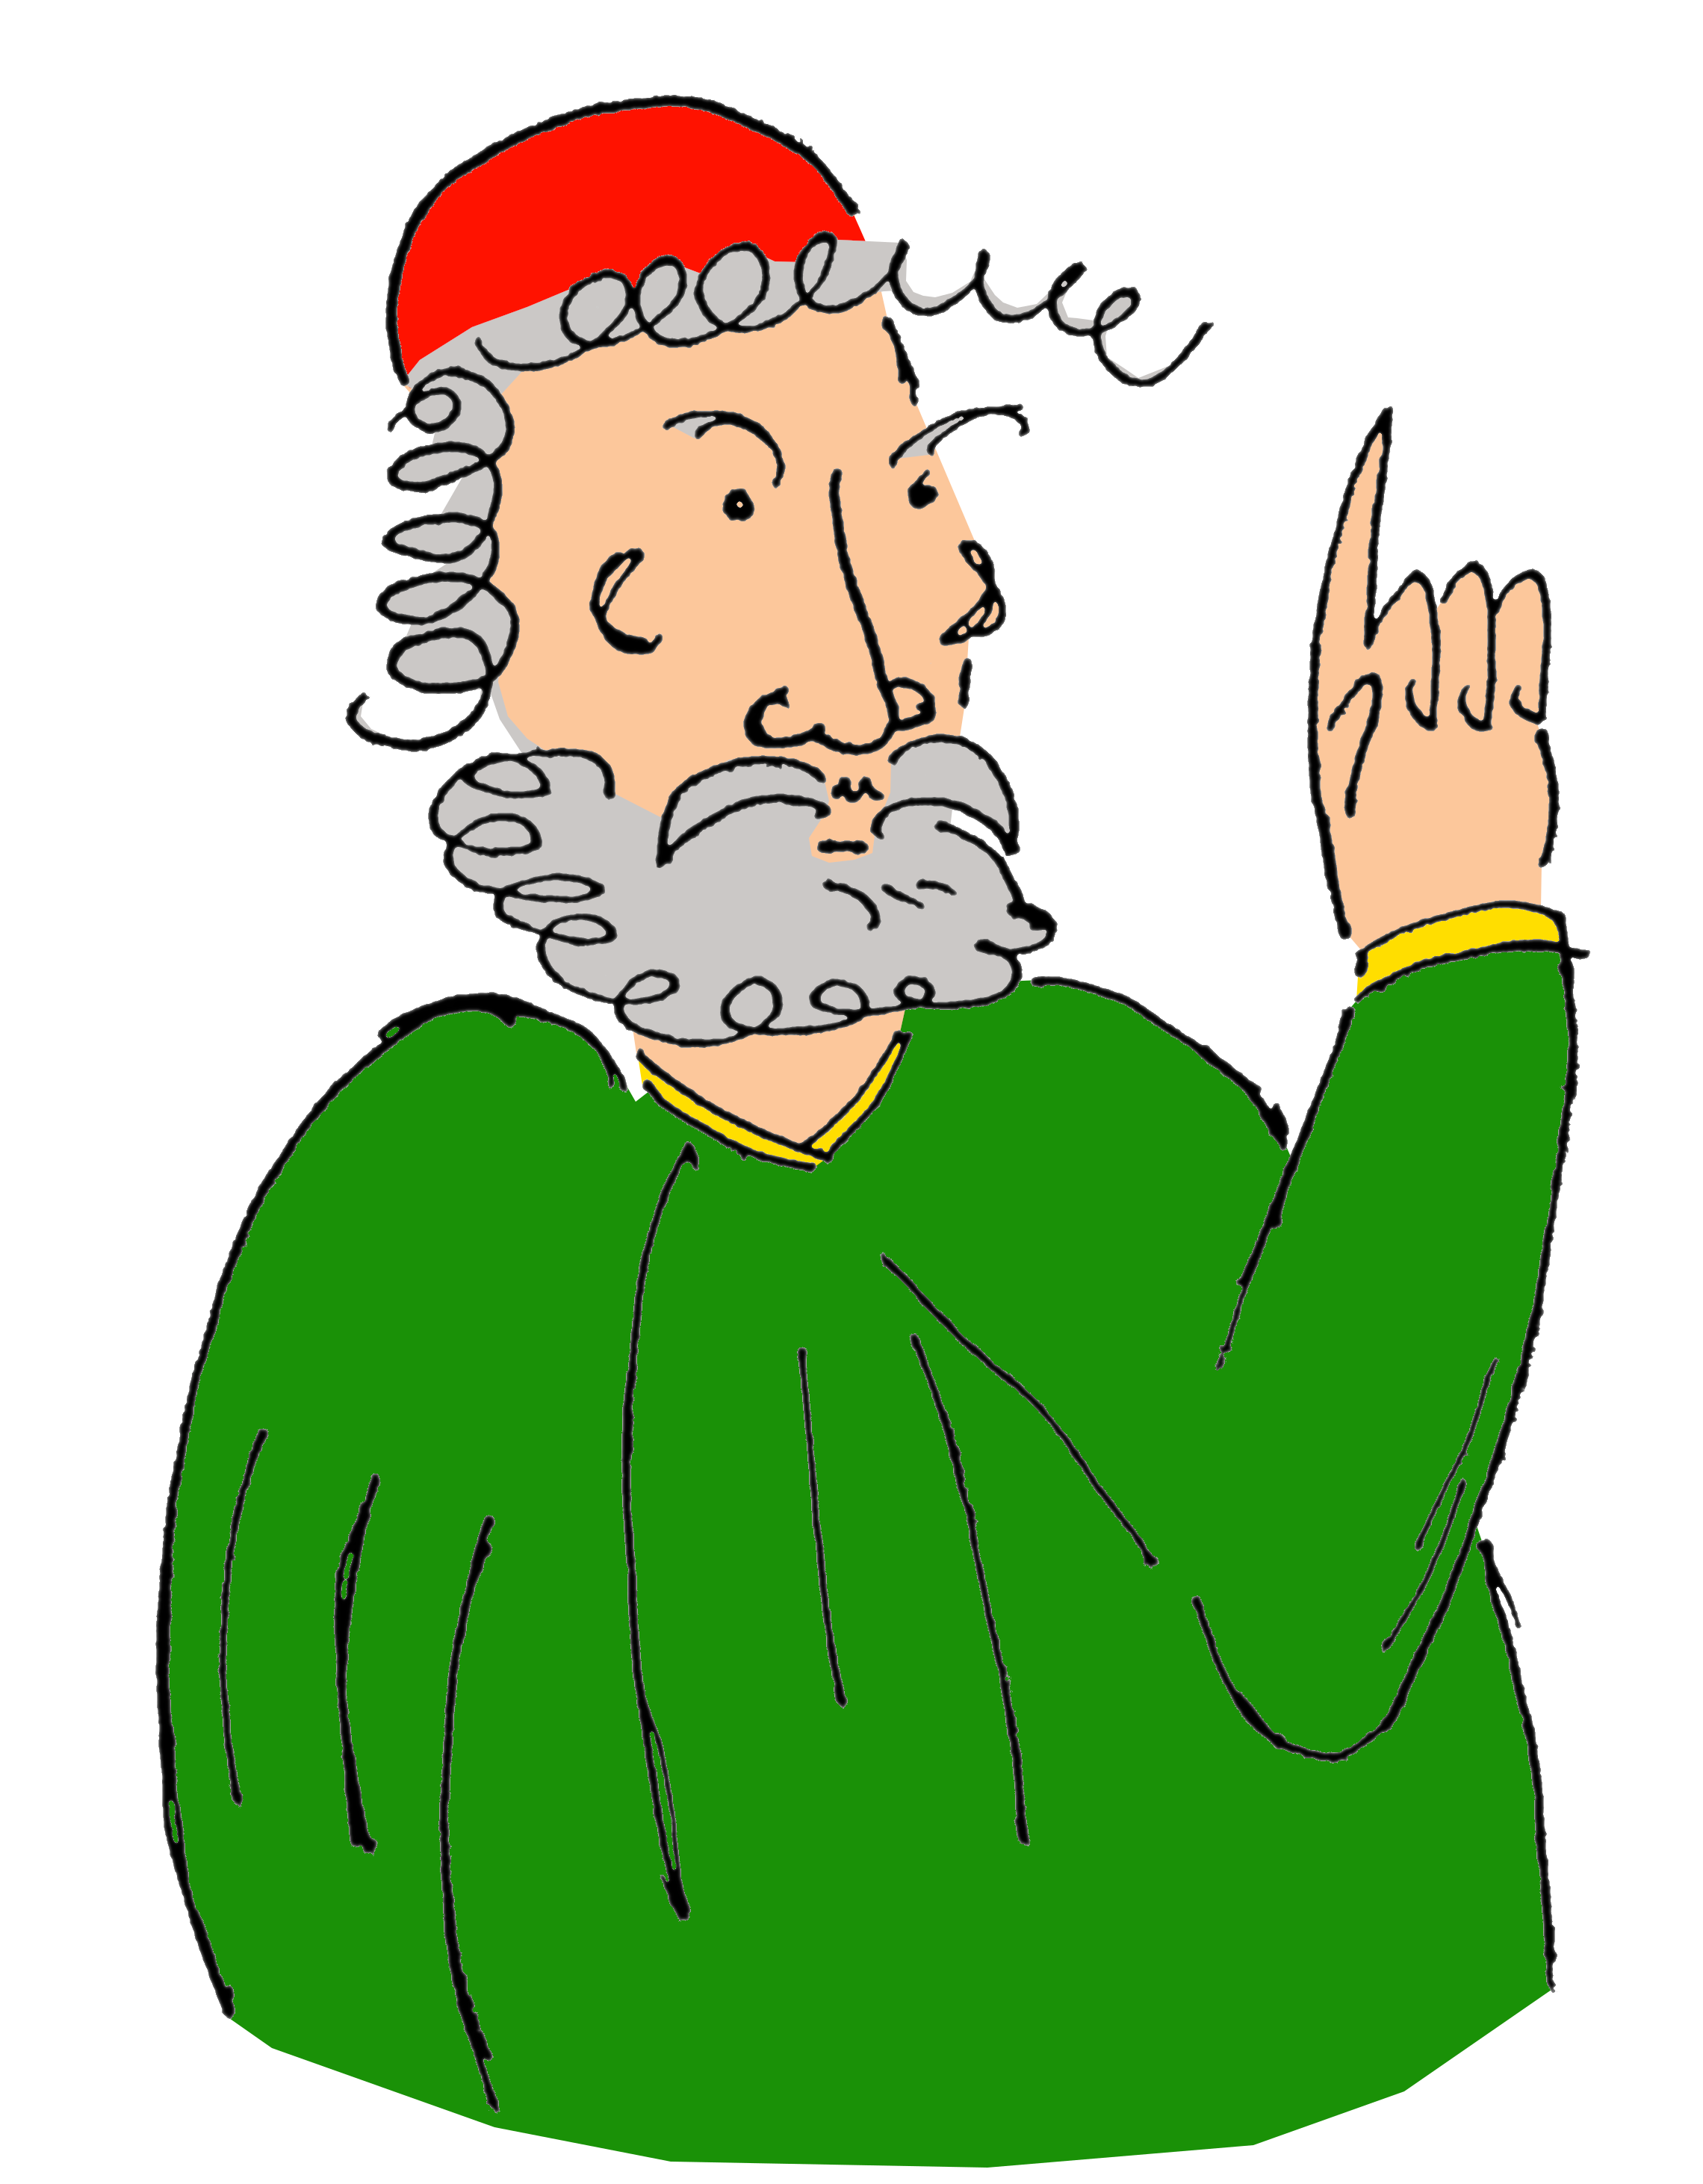
\includegraphics[width=8cm]{tolomeo}};
			\node (example-textwidth-2) [notice={(-3,0.5)}, ultra thick, right, align=center, text width=12cm, color=black, fill=white, font=\fontsize{23pt}{24pt}\selectfont] at (12,-1) {Qualunque errore ho fatto dipende da Ipparco!};
			\node (example-textwidth-2) [notice={(3,0.5)}, ultra thick, right, align=center, text width=12cm, color=black, fill=white, font=\fontsize{23pt}{24pt}\selectfont] at (12,-4) {Tolomeo! Sempre modesto, eh?!};
		\end{scope}
		%
		\begin{scope}[shift={(0,-42)}]
			\draw [ultra thick, fill=dida] (2.5,1.5) rectangle (28,-1.5);
			\node (example-textwidth-2) [right, align=left, text width=25cm, color=black, font=\fontsize{18pt}{19pt}\selectfont] at (3,0) {Il metodo più antico in assoluto è invece quello della parallasse, ovvero la misurazione simultanea da posizioni differenti dell'angolo tra la Luna e un dato punto di riferimento. };
		\end{scope}
		%
		\begin{scope}[shift={(0,-47)}]
			\node at (23,0) {
\includegraphics[width=5cm]{carl_sagan}};
			\node (example-textwidth-2) [notice={(3,0.5)}, ultra thick, right, align=center, text width=12cm, color=black, fill=white, font=\fontsize{23pt}{24pt}\selectfont] at (1,-1) {Ovviamente in questo modo risulta necessario sincronizzare tutti gli osservatori.};
		\end{scope}
		%
		\begin{scope}[shift={(0,-53.5)}]
			\draw [ultra thick, fill=dida] (2.5,2) rectangle (28,-2);
			\node (example-textwidth-2) [right, align=left, text width=24cm, color=black, font=\fontsize{18pt}{19pt}\selectfont] at (3,0) {Il metodo attualmente utilizzato risale al 1962, quando una squadra del MIT (\emph{Massachusetts Institute of Technology}) in collaborazione con gli astronomi sovietici dell'Osservatorio Astrofisico di Crimea portò a termine un esperimento per misurare il tempo di andata e ritorno di un impulso laser riflesso sulla superficie della Luna.};
		\end{scope}
		%
		\begin{scope}[shift={(0,-61)}]
			\draw[color=craterm, fill=moon, ultra thick] (6.5,0) circle (4.5cm);
			\foreach \x in {1,...,5}
			\draw [color=craterm, ultra thick, rotate around={72*\x:(6.5,0)}] (6.5,0) -- (6.5,2);
			\foreach \x in {1,3,...,20}
			\draw [color=craterm, ultra thick, rotate around={18*\x:(6.5,0)}] (6.5,0) -- (6.5,1.2);
			\foreach \x in {2,6,...,18}
			\draw [color=craterm, ultra thick, rotate around={18*\x:(6.5,0)}] (6.5,0) -- (6.5,0.9);
			\draw[fill=craterm, ultra thick] (6.5,0) circle (0.5cm);
			%down-sx
			\draw (3.3,-2.5) [rotate around={-45:(3.3,-2.5)}, color=linem,ultra thick,partial ellipse=20:160:1.5 and 0.5];
			\foreach \x in {0.01,0.02,...,0.1}
			\draw (3.3+\x,-2.5-\x) [rotate around={-45:(3.3,-2.5)}, color=craterm,ultra thick,partial ellipse=20:160:1.5 and 0.5];
			%down-dx
			\draw (9.7,-2.5) [rotate around={45:(9.7,-2.5)}, color=linem,ultra thick,partial ellipse=20:160:1 and 0.3];
			\foreach \x in {0.01,0.02,...,0.1}
			\draw (9.7+\x,-2.5-\x) [rotate around={45:(9.7,-2.5)}, color=craterm,ultra thick,partial ellipse=20:160:1 and 0.3];
			%up-sx
			\draw (3.5,3.2) [rotate around={45:(3.5,3.2)}, color=linem,ultra thick,partial ellipse=180:360:0.5 and 0.3];
			\foreach \x in {0.01,0.02,...,0.1}
			\draw (3.5+\x,3.2-\x) [rotate around={45:(3.5,3.2)}, color=craterm,ultra thick,partial ellipse=180:360:0.5 and 0.3];
			%up-dx shadow
			\draw (9.5,3) [rotate around={-50:(9.5,3)}, color=linem,ultra thick,partial ellipse=180:360:0.9 and 0.7];
			\foreach \x in {0.01,0.02,...,0.1}
			\draw (9.5+\x,3-\x) [rotate around={-50:(9.5,3)}, color=craterm,ultra thick,partial ellipse=180:360:0.9 and 0.7];
			%
			\draw[color=black, fill=earth, ultra thick] (20.5,-13) circle (7.2cm);
			%
			\draw [ultra thick, fill=space] (13.5,3) rectangle (26.5,-3);
			\node (example-textwidth-2) [right, align=left, text width=12cm, color=white, font=\fontsize{18pt}{19pt}\selectfont] at (14,0) {L'evoluzione di questo esperimento viene portato a termine grazie alle \emph{missioni Apollo} del 1969, quando gli astronauti posizionarono sulla superficie lunare degli specchi catarifrangenti, in modo tale da migliorare l'accuratezza della misura.};
			%
			\draw [ultra thick, fill=space] (0.5,-6.5) rectangle (13.5,-13.5);
			\node (example-textwidth-2) [right, align=left, text width=12cm, color=white, font=\fontsize{18pt}{19pt}\selectfont] at (1,-10) {I laser che viaggiano verso la Luna coinvolgono molteplici strutture e fanno parte del \emph{Lunar Laser Ranging}. La misura della distanza proveniente da questo progetto è di 384402 km con un errore di 1.1 millimetri, che in termini di tempo luce corrisponde a poco meno di 1.3 secondi.};
			%
			\draw [ultra thick, color=red] (8.5,-2) -- (18,-7);
		\end{scope}
		%
		\begin{scope}[shift={(0,-84)}]
			\draw [ultra thick, fill=dida] (14,5) rectangle (28,-5);
			\node (example-textwidth-2) [right, align=left, text width=13cm, color=black, font=\fontsize{18pt}{19pt}\selectfont] at (14.5,0) {Un metodo alternativo basato sullo stesso principio è quello di usare degli impulsi radar: nel 1957 lo \emph{US Naval Research Laboratory}, dopo aver inviato un segnale sulla superficie della Luna, ha rivelato quello di ritorno e misurato il tempo di ritardo, usato per ricavare la distanza dal nostro satellite. Purtroppo tale esperimento era soggetto a un errore eccessivamente alto e quindi il risultato prodotto non era considerato affidabile.};
			\draw [ultra thick, fill=earth!50!white] (1,-6) rectangle (29,-10);
			\node (example-textwidth-2) [right, align=left, text width=18cm, color=black, font=\fontsize{18pt}{19pt}\selectfont] at (10,-8) {L'esperimento venne ripetuto l'anno dopo, nel 1958, dal \emph{Royal Radar Establishment} in Gran Bretagna. La sintesi dei due risultati ha prodotto una misura pari a 384402 ± 1,2 km.};
		\end{scope}
		%
		\begin{scope}[shift={(5,-84)},scale=0.8]
			\begin{scope}
				\draw [fill=linem] (0,-11) [partial ellipse=180:360:4 and 0.8] -- (4,-11) -- (4,-9) -- (-4,-9) -- (-4,-11);
				\draw [fill=linem] (0,-9) [partial ellipse=0:360:4 and 0.8];
				\draw [fill=moon] (0,-9) [partial ellipse=180:360:3 and 0.5] -- (3,-9) -- (0,4) -- (-3,-9);
			\end{scope}
			%
			\begin{scope}[rotate around={-40:(0,0)}]
				\draw [fill=linem] (-3.5,1) -- (-2,-0.5) -- (2,-0.5) -- (3.5,1) -- (-3.5,1);
				\draw [fill=craterm] (0,0) circle (0.2 cm);
				\draw [fill=moon] (0,4.5) [partial ellipse=180:360:7.5 and 4];
				\draw [fill=linem](0,4.5) [partial ellipse=0:360:7.5 and 1];
				\draw [fill=craterm] (0,3.5) [partial ellipse=0:180:0.5 and 0.2];
				\draw [color=moon, line width=0.2 cm] (-4.5,4) -- (-0.4,9);
				\draw [color=moon, line width=0.2 cm] (4.5,4) -- (0.4,9);
				%
				\draw [fill=craterm] (0,9) [partial ellipse=180:360:0.5 and 0.2] -- (0.5,9) -- (0.5,10.5) -- (-0.5,10.5) -- (-0.5,9);
				\draw [fill=craterm] (0,10.5) [partial ellipse=0:360:0.5 and 0.2];
			\end{scope}
		\end{scope}
		%
		\begin{scope}[shift={(0,-100)}]
			\draw [ultra thick, fill=space] (1,-2) rectangle (29,2);
			\node (example-textwidth-2) [right, align=left, text width=15cm, color=white, font=\fontsize{18pt}{19pt}\selectfont] at (2,0) {Un altro sistema, meno preciso dei due precedenti, è quello delle occultazioni, ovvero quando la Luna passa davanti a una stella o a un pianeta.};
			\begin{scope}[shift={(15,0)}]
				\draw[color=black, fill=mars, ultra thick] (2.7,2.5) circle (0.2cm);
				\draw[color=craterm, fill=moon, ultra thick] (6.5,0) circle (4.5cm);
				\foreach \x in {1,...,5}
				\draw [color=craterm, ultra thick, rotate around={72*\x:(6.5,0)}] (6.5,0) -- (6.5,2);
				\foreach \x in {1,3,...,20}
				\draw [color=craterm, ultra thick, rotate around={18*\x:(6.5,0)}] (6.5,0) -- (6.5,1.2);
				\foreach \x in {2,6,...,18}
				\draw [color=craterm, ultra thick, rotate around={18*\x:(6.5,0)}] (6.5,0) -- (6.5,0.9);
				\draw[fill=craterm, ultra thick] (6.5,0) circle (0.5cm);
				%down-sx
				\draw (3.3,-2.5) [rotate around={-45:(3.3,-2.5)}, color=linem,ultra thick,partial ellipse=20:160:1.5 and 0.5];
				\foreach \x in {0.01,0.02,...,0.1}
				\draw (3.3+\x,-2.5-\x) [rotate around={-45:(3.3,-2.5)}, color=craterm,ultra thick,partial ellipse=20:160:1.5 and 0.5];
				%down-dx
				\draw (9.7,-2.5) [rotate around={45:(9.7,-2.5)}, color=linem,ultra thick,partial ellipse=20:160:1 and 0.3];
				\foreach \x in {0.01,0.02,...,0.1}
				\draw (9.7+\x,-2.5-\x) [rotate around={45:(9.7,-2.5)}, color=craterm,ultra thick,partial ellipse=20:160:1 and 0.3];
				%up-sx
				\draw (3.5,3.2) [rotate around={45:(3.5,3.2)}, color=linem,ultra thick,partial ellipse=180:360:0.5 and 0.3];
				\foreach \x in {0.01,0.02,...,0.1}
				\draw (3.5+\x,3.2-\x) [rotate around={45:(3.5,3.2)}, color=craterm,ultra thick,partial ellipse=180:360:0.5 and 0.3];
				%up-dx shadow
				\draw (9.5,3) [rotate around={-50:(9.5,3)}, color=linem,ultra thick,partial ellipse=180:360:0.9 and 0.7];
				\foreach \x in {0.01,0.02,...,0.1}
				\draw (9.5+\x,3-\x) [rotate around={-50:(9.5,3)}, color=craterm,ultra thick,partial ellipse=180:360:0.9 and 0.7];
			\end{scope}
			%
		\end{scope}
		%
		\begin{scope}[shift={(0,-110)}]
			\node at (4,0) {
\includegraphics[width=5cm]{carl_sagan}};
			\node (example-textwidth-2) [notice={(-3,0.5)}, ultra thick, right, align=center, text width=12cm, color=black, fill=white, font=\fontsize{23pt}{24pt}\selectfont] at (9,-1) {Con questo metodo gli astronomi \textbf{John O'Keefe} e \textbf{Pamelia Anderson} calcolarono nel 1952 un valore di 384407.6 ± 4.7 km. Questo risultato venne migliorato nel 1962 da \textbf{Irene Fischer} che ottenne un valore di 384403.7 ± 2 km.};
		\end{scope}
		%
		\begin{scope}[shift={(0,-117)}]
			\node at (27,0) () {
\includegraphics[width=3.7cm]{licenza}};
			\node at (18,-0.1) {\textcolor{black}{\fontsize{14}{15}\selectfont Testo e illustrazioni: @ulaulaman - Gianluigi Filippelli}};
		\end{scope}
	\end{tikzpicture}
%
\end{document}
